\documentclass{article} % say
\usepackage{tikz}
\usetikzlibrary{patterns}
\renewcommand{\familydefault}{\sfdefault} % for sans font
\begin{document}

% http://cremeronline.com/LaTeX/minimaltikz.pdf

\texttt{Bitmap.Optimize()} uses the values of cardinality (\texttt{c.n} or $N$) and
run count (\texttt{c.runCount()} or $N_R$) to convert container types, achieving minimal storage size, according to this diagram:\\

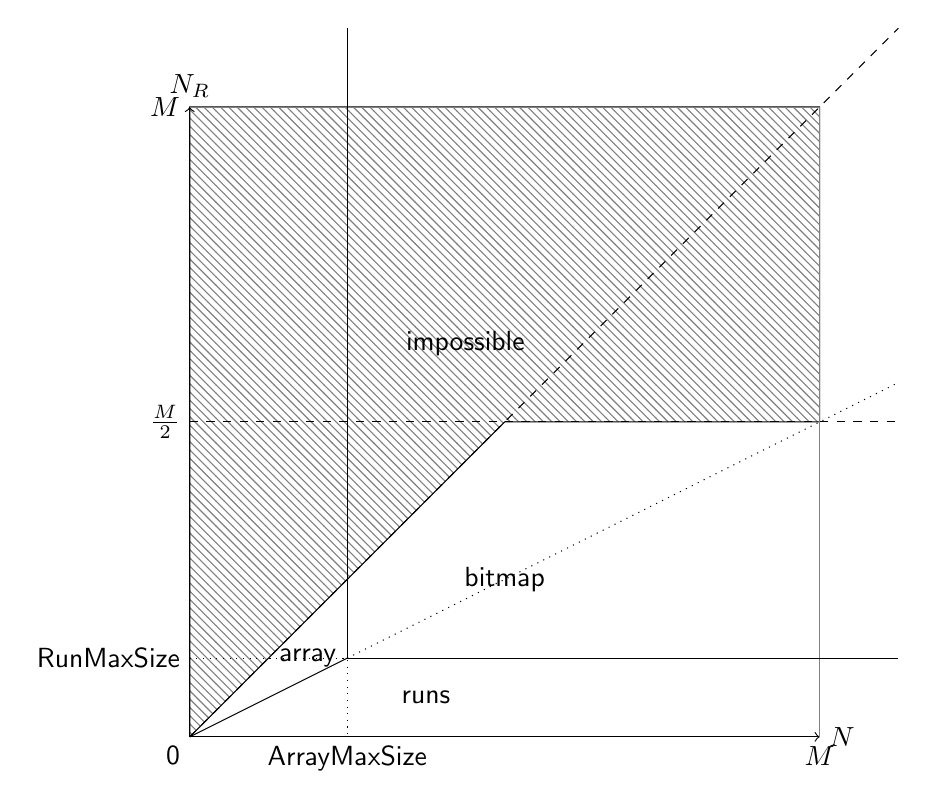
\begin{tikzpicture}
  \draw [pattern=north west lines, pattern color=gray] (0, 0) -- (4, 4) -- (8, 4) -- (8, 8) -- (0, 8) -- (0, 0);
  \draw [<->] (0,8) node [above] {$N_R$} node [left] {$M$} -- (0,0) node [below left] {0} -- (8,0) node [right] {$N$} node [below] {$M$};
  \draw [help lines] (8, 0) -- (8, 8) -- (0, 8);
  \draw [dotted] (0,1) node [left] {RunMaxSize} -- (2,1) -- (2,0) node [below] {ArrayMaxSize};
  \draw [solid] (9, 1) -- (2,1) -- (2,9);
  \draw [solid] (0, 0) -- (2, 1);
  \draw [dotted] (2, 1) -- (9, 4.5);
  \draw [dashed] (0, 0) -- (9, 9);
  \draw [dashed] (4, 4) -- (9, 4);
  \draw [dashed] (0, 4) -- (4, 4);
  \node at (1.5, 1) {array};
  \node at (3, .5) {runs};
  \node at (4, 2) {bitmap};
  \node at (3.5, 5) {impossible};
  \draw (0, 4) node [left] {$\frac{M}{2}$};
\end{tikzpicture}

$M$ is the maximum number of bits in a container.\\

Note the impossible region: The $N = N_R$ diagonal represents sets where every
bit is isolated - all run lengths are one. No set can be above this line. The
point $(\frac{M}{2}, \frac{M}{2})$ represents the set where alternating bits are
present, which represents the maximum number of runs for a fixed set size. No
set can be above this line. The remaining region represents all possible sets,
with container type regions separated by the solid lines.


\bigskip


Let $A$ be the array element size in bits, $R$ be the RLE start/end element size. Then array size is $AN$, run size is
$2RN_R$, and bitmap size is $M$.\\

Arrays are smaller than bitmaps when $AN < M$ or $N < \frac{M}{A} = ArrayMaxSize$.\\
Runs are smaller than bitmaps when $2RN_R < M$ or $N_R < \frac{M}{2R} = RunMaxSize$.\\
Array are smaller than runs when $AN < 2RN_R$ or $N < 2\frac{R}{A} N_R$.\\

Currently (v0.4.x), $A = R = 32$, $M = 65536$, so\\ 

$ArrayMaxSize = 2048$.\\
$RunMaxSize = 1024$.\\
Arrays are smaller than runs when $N < 2 N_R$.\\
\\
\begin{tabular}{l | c | c}
    & 32-bit & 16-bit \\
  \hline
  ArrayMaxSize & 2048 & 4096 \\
  \hline
  RunMaxSize & 1024 & 2048 \\
\end{tabular}

\end{document}

